\chapter{Conclusions}
\graphicspath{{conclusions/figs}}
\label{chapter:conclusions}

\lettrine[lines=3,loversize=0.1,findent=0.1em,nindent=0em]{I}{n} this thesis I set out to advance understanding of tipping points in the climate-carbon cycle system.
Below I summarize the findings of each of the research strands that have been presented in this thesis. I will then discuss potential avenues for further work.

\section{Research Conclusions}
\subsubsection{\nameref*{chapter:continuous_compost_bomb}}

In \cref{chapter:continuous_compost_bomb} I investigated the the effect of adding a vertical spatial dimension to a model of the compost bomb instability.
The purpose of this was twofold. 
Firstly, I was interested to see if the instability still existed in a more realistic model.
Secondly, I wanted to know if certain wildfires could be caused by biogeochemical heating and in order to do this more realistic physics was desirable.

In order to investigate this, I created a partial differential equation model of soil temperature which included biogeochemical heating. I made the assumption
that soil carbon could be viewed as being time invariant, which placed the model into the `compost bomb limit' of~\cite{Luke2011}. This came at the cost of preventing
R-tipping so the potential for B-tipping was investigated. Furthermore the effect of a large seasonal cycle in atmospheric temperatures on the soil was investigated.

It was shown that for sufficiently large atmospheric temperatures the model had no steady state. This meant that the soil temperatures had diverged and that a compost bomb
had occurred. If, as in the real world, soil carbon was allowed to evolve dynamically then the amount of soil carbon would decrease which would prevent the soil temperatures from diverging;
instead they would simply reach a large value.

It was also shown that a sufficiently large seasonal cycle --- which could be realised by a summer heat wave --- could be enough to trigger a compost bomb.
Furthermore, the size of the seasonal cycle was not dissimilar to the seasonal cycles observed in parts of Siberia in extreme years such as 2010, as shown in \cref{fig:seasonal_cycle_maps}.
This can be seen as evidence that Siberian wildfires may be caused, in part, by biogeochemical heating. 

\begin{figure}
  \centering
  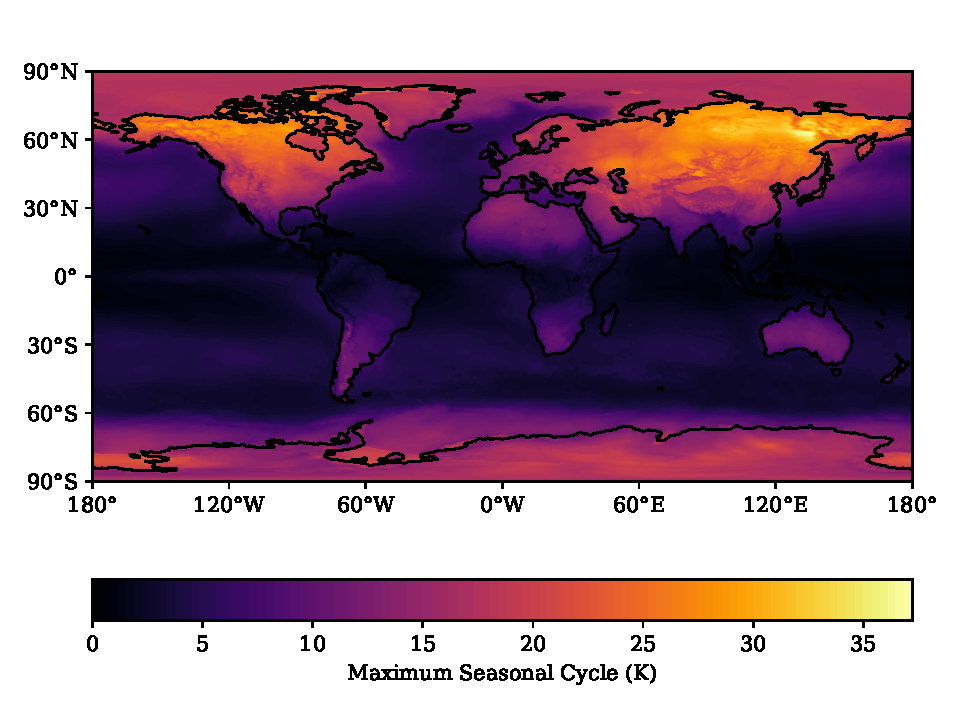
\includegraphics[width=\textwidth,keepaspectratio]{seasonal_cycles}
  \caption[Map of Seasonal Cycles]{The largest observed seasonal cycle in the ERA$5$ reanalysis \parencite{Hersbach2020} over the period 1940--2022.
    The magnitude of the seasonal cycle is defined as half the difference between the maximum and minimum monthly averaged \SI{2.0}{\meter} air temperatures.}
  \label{fig:seasonal_cycle_maps}
\end{figure}

Due to the approximation that soil carbon was constant in time, the compost bomb instability became an example of B-tipping rather than R-tipping. It does not necessarily
follow that the system would experience R-tipping if this approximation was relaxed. However, it is reasonable to assume that the vertical diffusion of heat would not be a barrier to
R-tipping, as long as the atmospheric temperatures were raised rapidly compared to the soil carbon timescale, due to the significant timescale separation between the soil thermal and
carbon timescales \parencite{Luke2011}.

The approximation that soil carbon is constant is accurate over the timescales of a year, given the multi-decadal turnover time of soil carbon \parencite{Varney2020}.
It follows therefore, that there can be good confidence in the conclusions drawn about the seasonal cycle. However, the applicability of the results to Siberian wildfires may be more doubtful.
This is because it may be better to view a hot summer period as a shorter perturbation to atmospheric temperatures, rather than an amplified sinusoid. This case has
since been studied by~\cite{OSullivan2023} for the model of~\cite{Luke2011}. They also found for realistic Siberian summer temperatures compost bombs were possible. 

To summarise, in \cref{chapter:continuous_compost_bomb} I managed to show that adding in the vertical diffusion of heat does not suppress the compost bomb. This therefore increases the confidence
that the effect is real. Furthermore I also showed that a hot summer, as modelled by a large seasonal cycle of temperature, could cause compost bombs, which suggests biogeochemical heating may
play a role in Siberian wildfires. A paper based on this chapter has been published as~\cite{Clarke2021}.

\subsubsection{\nameref*{chapter:global_bomb}}

The investigation into the role of biogeochemical heating in the carbon cycle was continued in \cref{chapter:global_bomb}. Instead of looking at the local effect of biogeochemical heating,
the effect at the global scale was considered. This was motivated by the fact that the extra carbon released by biogeochemical heating would increase atmospheric temperatures,
further increasing respiration and thus biogeochemical heating.
This positive feedback therefore increases the chances of a compost bomb occurring, and it is important to quantify.

In order to do this, the model of~\cite{Luke2011} was assumed to hold at the global scale, meaning quantities could be replaced with their globally averaged values. The air temperature
was set to scale logarithmically with atmospheric \ce{CO2}, which in turn was calculated through carbon conservation. The additional effect of \ce{CO2} fertilisation was considered,
by assuming Net Primary Productivity was a saturating function of atmospheric carbon. The role of the ocean was accounted for very simply, by assuming that a fixed fraction of
carbon emissions become ocean carbon, which is equivalent to scaling down the flux from the land to the atmosphere by a fixed amount.

First, the stability of this model was investigated. To do this its bifurcation diagram was computed and it was found that there was a bifurcation if the climate sensitivity was large enough
or the biogeochemical heating was strong enough. The model was simple enough that the location of the bifurcation point could be computed analytically. 

It was found that for realistic amounts of biogeochemical heating, only a small difference to the stability of the system was made. It was however striking, that when there was no
\ce{CO2} fertilisation, the system was unstable at comparatively low levels of climate sensitivity. These levels are low enough to be in the range of CMIP models. It is therefore interesting to note
that without \ce{CO2} fertilisation the Earth's carbon and thus climate system may not be stable.

This approach to analysing the role of biogeochemical heating has its problems. To begin with, as demonstrated in \cref{chapter:continuous_compost_bomb}, biogeochemical heating
can be important regionally, yet this global modelling approach greatly reduces its influence. For example, for some combination of climate sensitivity and biogeochemical heating
it could be the case that a region of the Earth has an unstable carbon cycle whereas the global analysis would give a stable carbon cycle. This is problematic as an instability in one
region of the Earth could propagate to give a global instability.

Other modelling assumptions are also suspect. For example, it was assumed that atmospheric temperatures adjust instantaneously to increases in atmospheric \ce{CO2}, but in
reality this process can take years \parencite{Rugenstein2019}. It was also assumed that the ocean could be modelled as absorbing a fixed fraction of carbon, an assumption that is
further investigated in \cref{chapter:conceptual_carbon_cycle}.

\Cref{chapter:global_bomb} set out to analyse the effect, at the global scale, of biogeochemical heating. Due to the problems caused by biogeochemical heating
being so regionally heterogeneous, firm conclusions cannot be drawn. However, more confidence can be had in the role \ce{CO2} fertilisation and climate-carbon
sensitivity play. \ce{CO2} fertilisation acts to destabilise the system with respect to biogeochemical heating, although it still plays a stabilising role
overall. The terrestrial carbon system is most unstable at higher values of the climate-carbon sensitivity and lower values of the \ce{CO2} fertilisation strength.

\subsubsection{\nameref*{chapter:conceptual_carbon_cycle}}

In \cref{chapter:global_bomb}, it was noted that the Earth's terrestrial carbon cycle was stable for only some values of the climate-carbon sensitivity and that at low
\ce{CO2} fertilisation this critical sensitivity was very low. \Cref{chapter:conceptual_carbon_cycle} took these ideas further to investigate which parameter combinations
were compatible with the reconstructed behaviour of atmospheric \ce{CO2} in the the pre-industrial Holocene epoch, which was a time of low \ce{CO2} variability.

In order to constrain the parameters a better ocean model was required than was used in \cref{chapter:global_bomb}. In \cref{chapter:conceptual_carbon_cycle}
the ocean carbon cycle from the IMOGEN model was used in addition to simplified box models. Biogeochemical heating was also not accounted for on the grounds
that \cref{chapter:global_bomb} had found the effect weak at the global scale.

Using the IMOGEN ocean carbon cycle model, it was found that there was a critical value of climate sensitivity beyond which the carbon cycle would become unstable.
The bifurcation appeared to be a Hopf bifurcation. The oscillations after the bifurcation had a large amplitude and are incompatible with the observed behaviour of the
carbon cycle.

Using a two box model, these results could be recreated. Furthermore, it could be confirmed that the bifurcation was a Hopf bifurcation and the bifurcation point
could be determined analytically. The two box model could give a Hopf bifurcation at the same point in parameter space as the IMOGEN model.

A one box model was also formulated, which could show a bifurcation of various types depending on the choice of the timescale of the box.
For a fast timescale, this was a transcritical bifurcation, similar to the system analysed in \cref{chapter:global_bomb}. Furthermore, because the bifurcation
point could be analytically computed, this can be compared to the bifurcation point derived in \cref{chapter:global_bomb} to give an interpretation to the
ocean model in that chapter. It was found that the ocean model in \cref{chapter:global_bomb} was self-consistent only when the ocean timescale was very short.

If the ocean box timescale was longer, the bifurcation would become a Hopf bifurcation. However the bifurcation point was at a different point in parameter space to that of the
bifurcation in IMOGEN.

The critical climate sensitivities found using the IMOGEN model were, for realistic values of \ce{CO2} fertilisation, around \SI{10}{\kelvin} which could be
related to equilibrium climate sensitivities around of \SI{6}{\kelvin}. These values are not substantially larger than those found in a number of CMIP$6$ \parencite{Zelinka2020}.
This raises the possibility that when performing coupled climate-carbon simulation some of these models may not be able to simulate a stable pre-industrial
period. Furthermore those models which have low enough climate sensitivity to be on the `correct' side of the bifurcation may still have unrealistic levels of \ce{CO2} variability
due to the phenomenon of critical slowing down. As climate models increase the complexity of their carbon cycle representations by including, for example,
nutrient limitation, the magnitude of the \ce{CO2} fertilisation effect may decrease \parencite{Wiltshire2021}, which would make these models more likely to be unstable.

The analysis in \cref{chapter:conceptual_carbon_cycle} ignored certain effects. It ignored the climate effect on net primary productivity, which is likely to weaken it
in the tropics where temperatures exceed the optimum temperatures for photosynthesis and strengthen it in the high latitudes where temperatures are currently
below optimum \parencite{Sage2007}.
However, this effect is small relative to the effect of \ce{CO2} fertilisation in most models \parencite{Arora2020}.
It also made the same assumptions about the instantaneous temperature equilibration to atmospheric \ce{CO2} as was made in \cref{chapter:global_bomb}.
Whilst this may effect the behaviour of the carbon cycle beyond the bifurcation point where \ce{CO2} is varying significantly;
it is unlikely to effect the position of the bifurcation much as \ce{CO2} levels are constant before the bifurcation and thus the equilibrium assumption is more reasonable.

In summary, \cref{chapter:conceptual_carbon_cycle} showed that certain parameter regimes were not compatible with the behaviour of \ce{CO2} over the Holocene.
This behaviour could not be recreated recreated using a one box model, but could be using a two box model. This suggests the importance of two timescales to the bifurcation.
Furthermore the critical parameter values identified are close to those in
some CMIP$6$ models suggesting that they would not be able to give a stable pre-industrial control simulation if run in a coupled climate-carbon configuration.

\subsubsection{\nameref*{chapter:spatial_ews}}

In the final portion of this thesis I was interested in examining early warning signals for tipping points when the usual assumptions made do not apply.
\Cref{chapter:spatial_ews} examined the case where the system is not forced slowly compared to its own timescale. This was of interest because anthropogenic climate change
occurs on relatively short timescales compared to the timescales of the Earth system, so there is reason to suspect that early warning signals may be less effective.

The use of spatial early warning signals was investigated. This was motivated by the fact that they give an `instantaneous' early warning signal and so do not have
to be calculated over a non-stationary time series. However, by introducing a spatial dimension into the system, the interaction between different spatial locations
need to be considered. This therefore lead to a numerical investigation of the reliability of early warning signals as a function of the rate of forcing and of the strength of
the spatial coupling.

To investigate this, a simple system with diffusive coupling was considered which depended on two parameters: the rate of forcing and the strength of the spatial coupling.
This system was identified as a mean field theory of the Ising ferromagnet, which enabled the use of techniques from the theory of phase transitions.

The reliability of both spatial and time series based early warning signals was calculated as a function of the two parameters.
It was found that spatial early warning signals were more reliable at larger rates of forcing than time series based early warning signals. However as the spatial coupling
strength increased this advantage decreased, until time series based early warning signals became more reliable for very strongly coupled systems. Arguments were given, in terms of the correlation
length and the distance from equilibrium in order to explain this dependence.

Although spatial early warning signals are reliable at increased rates of forcing compared to time series based early warning signals, they are still not reliable at rates which exceed
the timescale of the system itself. This suggests it may not be applicable to important Earth system tipping elements, such as the ice sheets, which have very slow time scales. Furthermore, the reliability decreases with
increasing spatial coupling which could be problematic for some tipping elements which have large-scale coherence. Whilst the coupling considered was the simplest \emph{local} coupling, non-local
coupling may be important in the climate system. Non-local couplings could act to increase the correlation length which would decrease the usefulness of spatial early warning signals further.

Overall however, this chapter extends the use of early warning signals to more rapidly forced systems. It also identifies a complementarity; spatial early warning signals are more reliable
for rapidly forced systems that are weakly coupled in space but time series based early warning signals are more reliable for slowly forced systems that are strongly coupled in space.
Given the vast quantity of remotely sensed spatial data available \parencite{Campbell2011} it is hoped that these techniques will be of use to researchers.

\subsubsection{\nameref*{chapter:rosa}}

In \cref{chapter:rosa}, I investigated the role of the assumptions made about the noise systems experience and how that affects early warning signals.
The typical assumption made is that the noise is white noise --- which means it has no temporal correlations. However when a system is forced over short timescales relative
to its own time scale, which is of relevance to climate change, temporal correlations become more important. Furthermore, there is no guarantee that these temporal
correlations are constant --- the stochastic process may not be stationary.

I investigated the effect of temporal correlations in the noise process by comparing early warning signals for a simple system, which could undergo a bifurcation, when subject to
white and red noise. It was found that in the presence of red noise the early warning signals were worse than in the case of white noise.

I then showed how, if there was some estimate of the noise, early warning signals could still be obtained for arbitrary noise processes. This could be done by moving to the frequency domain
where the effect of the noise process could be easily removed. I could verify numerically that the early warning signals obtained this way worked well for red and white noise processes.
Furthermore, in the case where the noise was not stationary, this method could still give good early warning signals.

I also applied this to the case of local Amazon dieback in CMIP$6$ models. It was found that the new method could give more early warning signals for abrupt transitions in Amazonia
when compared to more conventional early warning signals. The noise process was assumed to be given by the \SI{2}{\meter} air temperature; this gives evidence, along with
other work \parencite{Parry2022,Ritchie2022}, of the role air temperature plays in giving early warning signals about Amazon dieback.

The most obvious problem with this method is that it assumes the noise process is known. The correct choice of noise is not in necessarily known for all
tipping elements and as such relies on the scientific understanding of the problem. It also requires that the noise has been measured, thus requiring extra data compared to
conventional early warning signals. Additionally, it assumes a single noise source, whereas in reality the noise is likely to be a combination of multiple components.

\Cref{chapter:rosa} set out to investigate the role of temporal correlations play in early warning signals. It was able to demonstrate the importance of uncorrelated noise
for conventional early warning signals. Furthermore it was able to offer a way to avoid these problems, even in the case where the noise was non-stationary.
Whilst in some situations it may not be possible to use the method developed in \cref{chapter:rosa}, its usefulness was demonstrated in the case of Amazon dieback
where the method did perform well. A paper based on this chapter has been published as~\cite{Clarke2023}.


\section{Outlook}
One obvious future research direction would be to consider the effect of biogeochemical heating in a complex land surface model, such as JULES\@.
This would enable a more precise quantification of this process, taking into account the effect of spatially heterogeneous soil properties such as
soil moisture and changes in conductivity. Conductivity in particular was shown to have a significant control on the magnitude of the effect of biogeochemical heating.

Furthermore, the use of JULES, combined with forcing data sets would enable an investigation into Siberian wildfires. For example, 2020 was a year of unusually widespread
Siberian fires \parencite{Witze2020}. `Zombie', or over-winter, fires were identified as a possible cause. This is of interest because fires
caused by biogeochemical heating may manifest as zombie fires.
Furthermore, using future projections of climate change the changing probability of biogeochemical heating driven fires could be quantified.

It was noted that the investigation in \cref{chapter:global_bomb} could not capture the regional effects of biogeochemical heating. One way this investigation could be easily extended without
resorting to a complex land surface model is by considering a `two-region' model of soil carbon:
\begin{subequations}
  \label{eq:two_region_model}
  \begin{align}
    \dv{C_1}{t} &= \Pi_1(C_a) + \Pi_{c1} W\left(-\frac{r_1C_1}{\Pi_{c1}} \left(\frac{C_a}{C_{a0}}\right)^{\mu_1} \right) \\
    \dv{C_2}{t} &= \Pi_2(C_a) + \Pi_{c2} W\left(-\frac{r_2C_2}{\Pi_{c2}} \left(\frac{C_a}{C_{a0}}\right)^{\mu_2} \right) \\
  \end{align}
\end{subequations}
where $C_i$ are the soil carbon levels in region $i$, the parameters $\Pi_{ci}$ quantify the amount of biogeochemical heating and $\mu_i$ the climate-carbon sensitivity in that region. By assuming
$\Pi_{c1} \ll \Pi_{c2}$ this then models a region where biogeochemical heating is important, such as high latitude peatlands, coupled to a region where biogeochemical heating is less important,
which could represent the rest of the globe.

Another use for JULES could be to determine the bifurcation point which separates stable from unstable carbon cycles. To do this, it could be paired with IMOGEN to emulate both the
ocean carbon cycle as well as the effect of changes in atmospheric \ce{CO2} on surface temperatures. It seems likely that this JULES-IMOGEN combination would still experience the sort of
bifurcation described in \cref{chapter:conceptual_carbon_cycle}. This is because JULES has, at each grid square, essentially the same soil carbon dynamics as in \cref{chapter:conceptual_carbon_cycle}
and the ocean carbon cycle as simulated by IMOGEN will be same. However, changing the representation of ocean temperatures in IMOGEN may change the position of the bifurcation.
 
To extend the investigation into spatial early warning signals, more complex spatial coupling forms could be considered. Furthermore, the investigation was done in 1 dimension, it
would be interesting to look at the two and three dimensional case as the behaviour of spatial systems near the bifurcation point is known to be strongly dependent
on dimension \parencite{Stanley1999}. The ROSA method could also be extended by considering the multidimensional case in terms of both state and noise.

As \cref{chapter:spatial_ews} showed, for very rapidly forced systems early warning signals, even when calculated spatially, are not reliable. It would be useful therefore to
establish early warning signals for this regime. Indeed, given the possibility for overshooting tipping points \parencite{Ritchie2021}, it would be useful to create warning signals that could
indicated when a system has passed the tipping point but not yet transitioned to the new state. As this is a nonautonomous regime, few generic properties can be assumed. It may therefore be
most useful to investigate system specific early warning signals in this case.

\section{Summary}

The aim of this thesis was to examine instabilities in the climate-carbon system and adapt early warning signals to more climate relevant cases.
It extended the realism of models of biogeochemical heating by adding a spatial dimension, demonstrating its potential
relevance to some types of wildfire. Although this biogeochemical feedback was shown to be small at the global level, that analysis revealed that there are constraints on climate-carbon
system parameters. In particular, it showed that only certain values climate sensitivity and \ce{CO2} fertilisation strengths are compatible with the behaviour of \ce{CO2} over the Holocene.
Furthermore, these values are close to some values found in CMIP$6$ models, suggesting some of these models are at risk of being unrealistically unstable.

The theory of early warning signals was advanced, extending them to more realistic cases where the behaviour of the forcing matters --- either due to its time correlation structure
or because it is rapidly changing. In doing so I have drawn connections to the physics of phase transitions, the theory of which constitutes a rich body of research which I hope will provide
many insights in the future.